\newpage	
\def \currentAuthor {Florian Tipotsch}
	\section{Technologie für Webapp}
\begin{itemize}
	\item PHP - Für Webapp
	\item Html - Für Webapp 	
	\item MySql - Für Datenbanken
	\item \nameref{sec:YII2} - Für Webapp
	\item \nameref{sec:MVC} - Für Webapp
	\item \nameref{sec:CRUD} - Für Webapp
	\item REST - Für Datenbank, Webapp und Datenspeicherung
\end{itemize}
	\subsection{HTML - Hypertext Markup Language}
	HTML sind die Grundlagen für jede Website. Sie bilden die Grundstruktur jeder Webseite, und werden von Browsern dargestellt. HTML wird von dem World Wide Web Consortium (W3C) \cite{W3C} und dem Web Hypertext Application Technology Working Group (WHATWG) \cite{WHATWG} weiterentwickelt.
	
	Gute Ressourcen zum lernen und schreiben von HTML findet man auf w3schools.com \cite {W3schools}
	
	\subsection{Was ist Yii}
	Yii ist ein high Performance PHP Framework welches vor allem für die Entwicklung im Web2.0 eingesetzt wird. Web 2.0 fördert die User aktiv im Web mitzumachen. Diese können eigenen Beiträge erstellen und diese auf der Website anzeigen lassen. Mehr dazu im Kapitel \nameref{sec:YII2}\cite{Web_2}

	\subsubsection{Alternative zu Frameworks}
	Yii kann sehr weitreichend eingesetzt werden. Mit dem richtigen Wissen und Fähigkeiten kann man alles was mit einer PHP Seite möglich ist ganz einfach in Yii2 umsetzten.

Allerdings sind Frameworks nicht Administratoren freundlich da sie sehr viel Vorwissen erfordern um diese richtig zu implementieren. Einfacher zu implementieren sind CMS Systeme. Es gibt sehr viele Große CMS Systeme zum Beispiel:

\begin{itemize}
\item Joomla
\item Wordpress
\item Drupal
\item Contao
\end{itemize}

Diese haben wir auch schon im Unterricht besprochen und damit Websites erstellt. Vorteile sind vor allem die einfache Implementierung und rasche Einrichtung einer Website. Auch SEO wird von den CMS Systemen vereinfacht. Nachteile sind allerdings oft eingeschränkte Möglichkeiten und grenzen welches das CMS setzt.

\subsubsection{Warum haben wir uns für YII2 entschieden}

Der Hauptgrund warum wir uns gegen CMS Systeme entschieden haben sind die eingeschränkten Möglichkeiten die wir damit hätten. Bei YII2 können wir die gesamte Website nach unseren Bedarf zusammenstellen und auch so bearbeiten wie wir es wollen. Es war uns auch wichtig das wir nach modernen Entwurfsmustern arbeiten. Siehe \nameref{sec:MVC}.

Wir hätten uns auch für andere Frameworks entscheiden können allerdings war uns Yii2 schon bekannt und wir haben damit schon einige Websites erstellt.

Alternativen für Yii2 sind:

\begin{itemize}
	\item PureMVC
	\item Laravel
\end{itemize}

\subsection{PureMVC}
PureMVC ist seit dem Release in 2008 unverändert. Das hat den Vorteil das der administrative aufwand sehr gering ist aufgrund nicht vorhandener Updates. Außerdem muss man das Framework nur einmal lernen und kann dieses dann meistern ohne irgendwelche Änderungen zu befürchten.
Es gibt auch Best-Practicse Beispiele in vielen verschiedenen Sprachen. Diese findet man auf der Website \cite{Pure_MVC}

\subsection{Laravel}
Laravel


\newpage
\def \currentAuthor{Kevin Glatz}


\section{Gas-Sensoren}

\subsection{MQ Gas Sensoren}
Es gibt mehrere MQ Gas Sensoren zum Beispiel:

\begin{itemize}
\item {MQ2}
	Methane, Butane, LPG, smoke
\item {MQ3}
	Alcohol, Ethanol, smoke
\item {MQ4}
	Methane, CNG Gas
\item {MQ5}
	Natural gas, LPG
\item {MQ6}
	LPG, butane gas
\item {MQ7}
	Carbon Monoxide
\item {MQ8}
	Hydrogen Gas
\item {MQ9}
	Carbon Monoxide, flammable gasses
\item Mehr gibt es auf der Website: \cite{MQ_Sensoren}
\end{itemize}

In der Schule haben wir den MQ2 zur Verfügung stehend werden wir auch von der Schule den Adafruit CCS811 bereitgestellt bekommen. Wir bedanken uns dafür vielmals.
\newline
{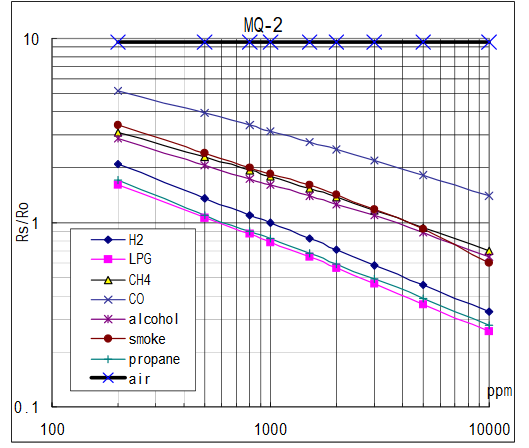
\includegraphics[width=0.8\linewidth]{figures/DatasheetMQ2.png}}{\cite{MQ_Datasheet}}

\cite{MQ_Sensoren}
\newline 

Im Datasheet \cite{MQ_Datasheet} kann man herauslesen das der Sensor MQ2 \cite{MQ_Sensoren} H2, LPG, CH4, CO, Alkohol, Rauch und Propan in einem Bereich von 200 bis 10000 Parts per million (Anteil pro Million) messen kann. Wie empfindlich der Sensor ist, hängt von den RS und RO werten ab.

\begin{itemize}
	\item RS: Sensor Widerstand bei verschiedenen Konzentrationen von Gas
	\item RO: Sensor Widerstand bei 1000ppm von H2 bei sauberer Luft.
\end{itemize}

\subsection{Adafruit CCS811}

